\documentclass[11pt]{article}

% ---------- Packages ----------
\usepackage[margin=1in]{geometry}
\usepackage{amsmath,amsthm,graphicx,enumitem,amssymb}
\usepackage{mathtools}
\usepackage{physics}        % derivatives, bras/kets, etc.
\usepackage{siunitx}        % units
\usepackage{graphicx}       % figures
\usepackage{float}          % figure placement
\usepackage{booktabs}       % nice tables
\usepackage{enumitem}       % better lists
\usepackage{fancyhdr}       % header/footer
\usepackage{titlesec}       % section formatting
\usepackage{hyperref}       % links
\usepackage{tcolorbox}      % boxes for answers
\usepackage{listings}       % code (MATLAB, Python, etc.)
\usepackage{xcolor}
\usepackage{bbm}        % blackboard bold italic
\usepackage{xcolor}
\usepackage{tikz}

% Define colors
\definecolor{codegreen}{rgb}{0,0.6,0}
\definecolor{codepurple}{rgb}{0.58,0,0.82}
\definecolor{backcolour}{rgb}{0.95,0.95,0.92}

% ---------- Hyperref Setup ----------
\hypersetup{
    colorlinks=true,
    linkcolor=blue,
    urlcolor=blue,
    citecolor=blue
}

% ---------- Header/Footer ----------
\pagestyle{fancy}
\fancyhf{}
\lhead{\textbf{\course}}
\rhead{\textbf{\assignment}}
\cfoot{\thepage}

% ---------- Custom Commands ----------
\newcommand{\course}{ASEN 5264 - DMU}
\newcommand{\assignment}{Homework \#5}
\newcommand{\studentname}{Bijan Jourabchi}

\newcommand{\R}{\mathbb{R}}
\newcommand{\E}{\mathbb{E}}
\newcommand{\Var}{\mathrm{Var}}
\newcommand{\Cov}{\mathrm{Cov}}

% Boxed answer environment
\newtcolorbox{answerbox}{
    colback=gray!5,
    colframe=gray!50,
    title=Answer,
    fonttitle=\bfseries
}

% Problem section format
\titleformat{\section}{\large\bfseries}{Problem \thesection:}{0.5em}{}

% ---------- Code Style ----------
\lstset{
    basicstyle=\ttfamily\small,
    keywordstyle=\color{blue},
    commentstyle=\color{green!50!black},
    stringstyle=\color{orange},
    breaklines=true,
    frame=single,
    extendedchars=true,
    literate={π}{{$\pi$}}1 {γ}{{$\gamma$}}1
}

% ---------- Document ----------
\begin{document}

% ---------- Title Block ----------
\begin{center}
    {\LARGE \textbf{\course}} \\[6pt]
    {\Large \assignment} \\[10pt]
    \studentname \\
\end{center}

\vspace{1em}
\hrule
\vspace{1em}

% Define Julia language manually
\lstdefinelanguage{Julia}{
  keywords={abstract, break, case, catch, const, continue, do, else, elseif,
      end, export, false, for, function, global, if, import, in, let, local,
      macro, module, otherwise, quote, return, struct, switch, true, try,
      type, typealias, using, while, mutable},
  keywordstyle=\color{blue}\bfseries,
  comment=[l]{\#},
  morecomment=[n]{\#=}{=\#},
  commentstyle=\color{codegreen}\ttfamily,
  stringstyle=\color{codepurple}\ttfamily,
  morestring=[b]',
  morestring=[b]"
}

% General Listing Settings
\lstset{
    language=Julia,
    backgroundcolor=\color{backcolour},   
    basicstyle=\ttfamily\small,
    breaklines=true,                 
    numbers=left,                    
    numbersep=5pt,                  
    frame=single
}

% =====================================================
\section{}

\begin{enumerate}[label = \alph*)]
    \item
        \begin{figure}[H]
                \centering
        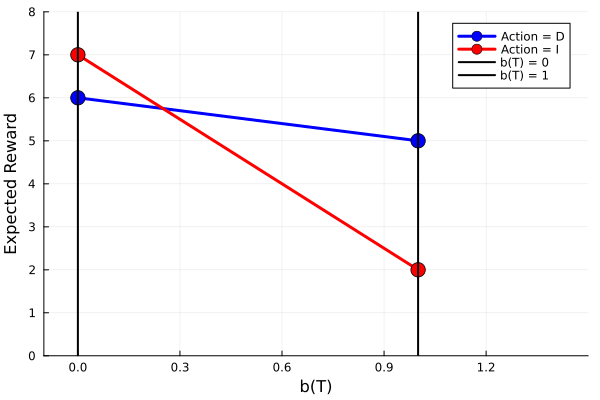
\includegraphics[width=\textwidth, height=0.25\textheight, keepaspectratio]{one_step.png}
        \caption{One Step $\alpha$-vector}
        \end{figure}
    \item
        With $b(T) = 0.6$, the optimal one step plan is to go with a domestic supplier.
        \begin{align*}
            \vec{R}^D &= \begin{bmatrix}
                6 \\ 5
            \end{bmatrix} \quad
            \vec{R}^I = \begin{bmatrix}
                9 \\ 2
            \end{bmatrix} \quad
            \vec{b} = \begin{bmatrix}
                0.4 \\ 0.6
            \end{bmatrix} \\
            \vec{R}^D \cdot \vec{b} &= 5.4 \quad \vec{R}^I \cdot \vec{b} = 4.8
        \end{align*}

        Since $\vec{R}^D \cdot \vec{b} > \vec{R}^I \cdot \vec{b}$, the action $a = D$ is the optimal action in the one step lookahead.
    \item
        As computed in part b, the expected reward given her belief is $5.4$.
    \item
        
        \begin{center}
            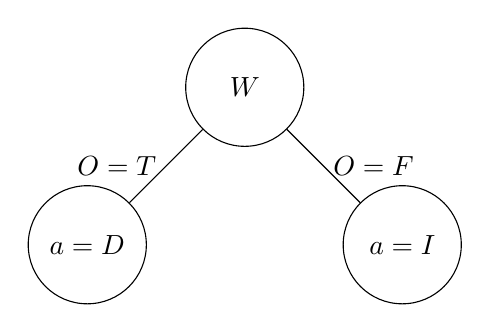
\begin{tikzpicture}[
                every node/.style={align=center},
                main node/.style={draw, circle, minimum size=1.5cm},
                edge/.style={-}
            ]

            % Nodes
            \node[main node] (W) at (0,2) {$W$};
            \node[main node] (D) at (-2,0) {$a =D$};
            \node[main node] (I) at (2,0) {$a =I$};

            % Edges
            \draw[edge] (W) -- node[midway,left,draw=none,fill=none] {$O = T$} (D);
            \draw[edge] (W) -- node[midway,right,draw=none,fill=none] {$O = F$} (I);

            \end{tikzpicture}
        \end{center}
    \item 
        
        Before we can plot the two step $\alpha$-vector, we must find the two step utility given by the following expression
        \[\mathcal{U}^\pi(s) = R(s,\pi) + \sum_{s'}T(s' \mid s, \pi) \sum_o \mathcal{O}(o \mid \pi, s') \mathcal{U}^{\pi(o)}(s')\]
        Where $\mathcal{U}^{\pi(o)}(s')$ is the one step alpha vector for action $\pi(o)$ is state $s'$.
        Evaluating, we get 
        \begin{align*}
            \mathcal{U}^\pi(F) &= -1 + [T(F \mid F, \pi) (\mathcal{O}(T \mid \pi, F) \mathcal{U}^{\pi(T)}(F) + \mathcal{O}(F \mid \pi, F) \mathcal{U}^{\pi(F)}(F)) + \dots \\
            &T(T \mid F, \pi) (\mathcal{O}(T \mid \pi, T) \mathcal{U}^{\pi(T)}(T) + \mathcal{O}(F \mid \pi, T) \mathcal{U}^{\pi(F)}(T))] \\
            &= -1 + \mathcal{U}^{\pi(F)}(F) = -1 + 9 = 8 \\
            \mathcal{U}^\pi(T) &= -1 + [T(F \mid T, \pi) (\mathcal{O}(T \mid \pi, F) \mathcal{U}^{\pi(T)}(F) + \mathcal{O}(F \mid \pi, F) \mathcal{U}^{\pi(F)}(F)) + \dots \\
            &T(T \mid T, \pi) (\mathcal{O}(T \mid \pi, T) \mathcal{U}^{\pi(T)}(T) + \mathcal{O}(F \mid \pi, T) \mathcal{U}^{\pi(F)}(T))] \\
            &= -1 + \mathcal{U}^{\pi(T)}(T) = -1 + 5 = 4
        \end{align*}

        Thus, the two step $\alpha$-vector is 
        \[ \vec{\alpha} =
        \begin{bmatrix}
            8 \\ 4
        \end{bmatrix}
        \]
        \begin{figure}[H]
                \centering
        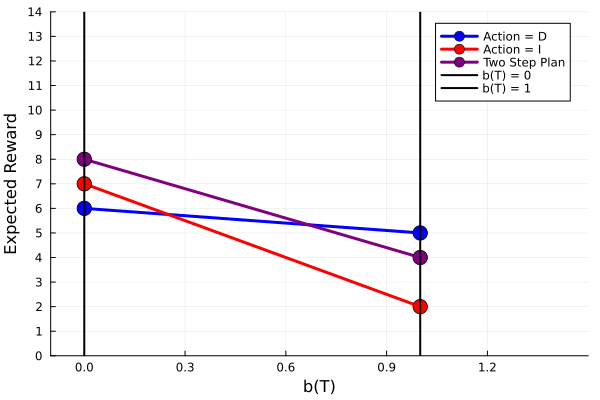
\includegraphics[width=\textwidth, height=0.25\textheight, keepaspectratio]{two_step.png}
        \caption{Two Step $\alpha$-vector}
        \end{figure}
    \item
        From our plot, it is evident that the two step plan is optimal plan. To find the expected reward, we will follow the same process as part b.
        \begin{align*}
            \vec{b} &= \begin{bmatrix}
                0.5 \\ 0.5
            \end{bmatrix} \quad \vec{R}^D = \begin{bmatrix}
                6 \\ 5
            \end{bmatrix} \quad
            \vec{R}^I = \begin{bmatrix}
                9 \\ 2
            \end{bmatrix} \quad \vec{R}^W = \begin{bmatrix}
                8 \\ 4
            \end{bmatrix} \\
            \vec{R}^D \cdot \vec{b} &= 5.5 \quad \vec{R}^I \cdot \vec{b} = 5.5 \quad \vec{R}^W \cdot \vec{b} = 6
        \end{align*}
        So, the two step plan has an expected reward of $6$.
    \item  
        If Jill had a preferance to support domestic suppliers, the problem could change considerably. For one, the reward for choosing $a = D$ could have larger rewards in either state.
        If the rewards for $a = D$ where large enough, it wouldn't even matter what the state is, choosing the domestic supplier will always be better. In this case, the one step plan for $a = D$ would be the optimal policy for any belief.
\end{enumerate}




% =====================================================
\section{}

With 10,000 MC trials, I get an average return of 38.72 for this POMDP. This can be interpreted as it taking on average 38 steps in the environment until the patient dies, since choosing the wait action always results in a reward of 1.

\begin{lstlisting}
using QuickPOMDPs: QuickPOMDP
using POMDPTools: Deterministic, Uniform, SparseCat, FunctionPolicy, RolloutSimulator, stepthrough, RandomPolicy
using Statistics: mean
using POMDPs: simulate
import POMDPs

cancer = QuickPOMDP(
        states = ["Healthy","ISC", "IC", "Death"],
        actions = ["wait","test","treat"],
        observations = ["positive","negative"],
        initialstate = Deterministic("Healthy"),
        discount = 0.99,

        transition = function(s,a)
            if s == "Healthy"
                return SparseCat(["Healthy", "ISC"], [1-0.02, 0.02])
            elseif a == "treat" && s == "ISC"
                return SparseCat(["Healthy", "ISC"],[0.6,0.4])
            elseif a != "treat" && s == "ISC"
                return SparseCat(["IC","ISC"],[0.1,0.9])
            elseif a == "treat" && s == "IC"
                return SparseCat(["IC","Healthy","Death"],[0.6,0.2,0.2])
            elseif a != "treat" && s == "IC"
                return SparseCat(["IC","Death"],[0.4,0.6])
            elseif s == "Death"
                return Deterministic("Death")
            end
        end,

        observation = function(s,a,sp)
            if a == "test"
                if sp == "Healthy"
                    return SparseCat(["positive","negative"],[0.05,0.95])
                elseif sp == "ISC"
                    return SparseCat(["positive","negative"],[0.8,0.2])
                elseif sp == "IC"
                    return SparseCat(["positive","negative"],[1.0,0])
                end
            end
            if a == "treat"
                if sp == "ISC" || sp == "IC"
                    return SparseCat(["positive","negative"],[1.0,0])
                end
            end

            return SparseCat(["positive","negative"],[0,1.0])
        end,

        reward = function(s,a)
            if s == "Death"
                return 0
            end
            if a == "wait" return 1.0 end
            if a == "test" return 0.8 end
            if a == "treat" return 0.1 end
        end
)



const policy = FunctionPolicy(o->"wait")
sim = RolloutSimulator(max_steps=100)
@show mean(POMDPs.simulate(sim, cancer, policy) for _ in 1:10_000)


\end{lstlisting}


% =====================================================
\section{}

I chose to implement DQN for my deep RL algorithm. While for the most part, my DQN was a standard approach to the algorithm, there were a few design decisions I made so that the algorithm achieved an expected reward above 40.
One of these decisions was to implement a warmup period before training the neural network. My idea was that this should give the model more time to explore actions freely, and will ensure the network has enough data before it began training.
In an attempt to improve performance, I implemented a method that saves the best Q-network seen throughout all the episodes. The code would then train the other networks on this Q network. That change allowed my implementation of DQN to reach a best score of 53.4.

\begin{figure}[H]
    \centering
    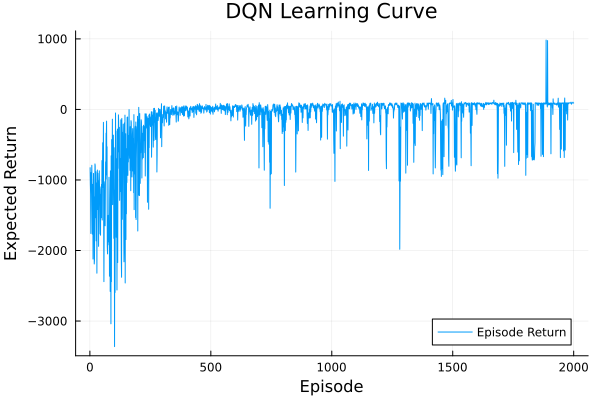
\includegraphics[width=\textwidth, height=0.25\textheight, keepaspectratio]{DQN_LC.png}
    \caption{DQN Learning Curve}
\end{figure}

\begin{lstlisting}
using DMUStudent.HW5: HW5, mc
using QuickPOMDPs: QuickPOMDP
using POMDPTools: Deterministic, Uniform, SparseCat, FunctionPolicy, RolloutSimulator
using Statistics: mean
using CommonRLInterface
using Flux
using Random
using ProgressMeter
using CommonRLInterface.Wrappers: QuickWrapper
using ElectronDisplay
ElectronDisplay.CONFIG.single_window = true
import POMDPs


env = QuickWrapper(HW5.mc,
                   actions=[-1.0, -0.5, 0.0, 0.5, 1.0],
                   observe=mc->observe(mc)[1:2])

function loss(Q, Q_target, s, a_ind, r, sp, done)
    if ! done
        return (r + 0.99*maximum(Q_target(sp)) - Q(s)[a_ind])^2
    else return (r-Q(s)[a_ind])^2 end
end

function policy(env,s,eps,Q)
    if rand() < eps
        return rand(1:length(actions(env)))
    else
        
        return argmax(i -> Q(s)[i], 1:length(actions(env)))
    end
end

function simulate(env,Q)
    reset!(env)
    r_tot = 0
    done = false
    count = 0
    eps = 0
    MAX_STEPS = 1000

    while !done && count < MAX_STEPS
        s = observe(env)
        a_ind = policy(env,s,eps, Q)
        r = act!(env, actions(env)[a_ind])
        sp = observe(env)
        done = terminated(env)
        r_tot += (0.99^count) * r
        s = sp
        count += 1
    end
    return r_tot / count
end

function dqn(env)
    Q = Chain(Dense(2,128), relu,
            Dense(128, length(actions(env)))) # Tune as needed
    opt = Flux.setup(ADAM(0.0005), Q)

    Q_target = deepcopy(Q)
    N_EPSISODES = 2000
    MAX_STEPS = 10000
    WARMUP_STEPS = 2000 # Idea is to let it explore for a while to gain experience_tuples before training to ensure NN has data
    REPLAY_CAPACITY = 200_000
    TRAIN_SAMPLES_PER_EPISODE = 2_000

    buffer = []
    learning_curve = Float64[]
    

    @showprogress for i = 1:N_EPSISODES
        
        reset!(env)
        count = 0
        eps = max(0.01, 1-i/N_EPSISODES)
        episode_return = 0
        done = false

        while !done && count < MAX_STEPS
            # Create our experience tuple
            s = observe(env)
            a_ind = policy(env,s,eps,Q)
            r = act!(env, actions(env)[a_ind])
            sp = observe(env)
            done = terminated(env)
            episode_return += r
            experience_tuple = (s, a_ind, r, sp, done)
            push!(buffer, experience_tuple)
            if length(buffer) > REPLAY_CAPACITY
                popfirst!(buffer) # drop oldest transition
            end
             
            count += 1
        end
        
        ## Save deepcopy only if Q policy is better than prev Q
        r_now = simulate(env,Q)
        
        push!(learning_curve, episode_return)
        r_trial = simulate(env,Q_target)

        if r_now > r_trial # This will ensure Q_target is always a better Q than the previous one
            
            Q_target = deepcopy(Q)

        end
        
        Q_target = deepcopy(Q)

        if length(buffer) >= WARMUP_STEPS
            n_updates = min(TRAIN_SAMPLES_PER_EPISODE, length(buffer))
            for data in rand(buffer, n_updates)
                # this runs a forward and backward pass to calculate the loss and gradient
                loss_value, grads = Flux.withgradient(loss, Q, Q_target, data...)

                # this will take a gradient step
                Flux.update!(opt, Q, grads[1])
            end
        end

        ## Stuff for learning curve
    end
    return Q, learning_curve
end

Q, learning_curve = dqn(env)

scr = HW5.evaluate(s->actions(env)[argmax(Q(s[1:2]))], n_episodes=10_000).score
println("\n score = $scr")
#if scr > 40
#    HW5.evaluate(s->actions(env)[argmax(Q(s[1:2]))], "bijan.jourabchi@colorado.edu") # you will need to remove the n_episodes=100 keyword argument and add your email as a positional argument to create a json file; evaluate needs to run 10_000 episodes to produce a json
#end
#----------
# Rendering
#----------

# You can show an image of the environment like this (use ElectronDisplay if running from REPL):
ElectronDisplay.display(render(env))

# The following code allows you to render the value function
using Plots
lc_plot = plot(
    1:length(learning_curve),
    learning_curve,
    xlabel="Episode",
    ylabel="Expected Return",
    title="DQN Learning Curve",
    label="Episode Return"
)
savefig(lc_plot, "DQN_LC.png")

xs = -3.0f0:0.1f0:3.0f0
vs = -0.3f0:0.01f0:0.3f0
heatmap(xs, vs, (x, v) -> maximum(Q([x, v])), xlabel="Position (x)", ylabel="Velocity (v)", title="Max Q Value")

\end{lstlisting}
\end{document}
